\documentclass{article}
\usepackage[utf8]{inputenc}
\usepackage{tikz}
\usetikzlibrary{shapes.geometric,arrows}

\tikzstyle{startstop} = [rectangle,rounded corners, minimum width=3cm,minimum height=1cm,text centered, draw=black,fill=red!30]
\tikzstyle{io} = [trapezium, trapezium left angle = 70,trapezium right angle=110,minimum width=3cm,minimum height=1cm,text centered,draw=black,fill=blue!30]
\tikzstyle{process} = [rectangle,minimum width=5cm,minimum height=1cm, text centered, text width =5cm,draw=black,fill=orange!30]
\tikzstyle{decision} =[diamond,minimum width=5cm,minimum height=0.5cm,text width =3cm, text centered,draw=black,fill=green!30]
\tikzstyle{arrow} = [thick,->,>=stealth]

\begin{document}

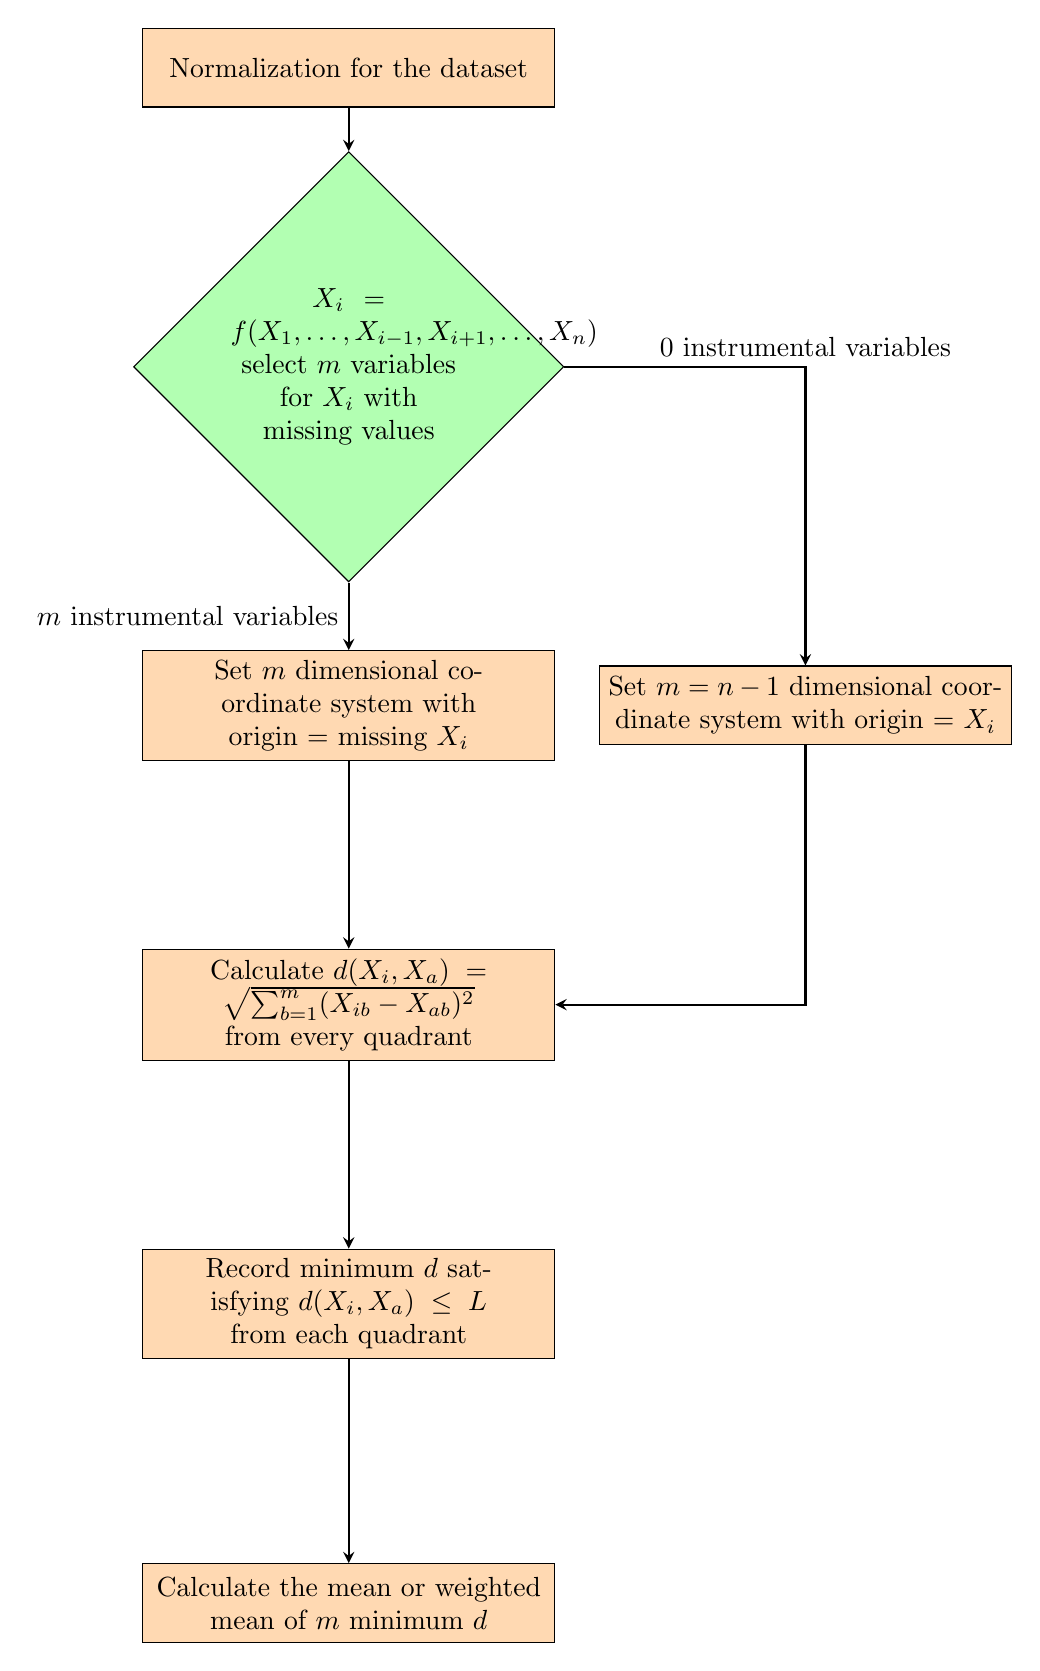
\begin{tikzpicture}[node distance = 3.8cm]

% \node (start) [startstop] {Start};
% \node (in1) [io] {Input};
\node(pro1) [process] {Normalization for the dataset};
\node(dec1) [decision, below of=pro1] {$X_{i} = f(X_{1}, \dots, X_{i-1}, X_{i+1}, \dots, X_{n})$ select $m$ variables for $X_{i}$ with missing values} ;
\node(pro2a) [process, below of=dec1, yshift = -0.5cm] {Set $m$ dimensional coordinate system with origin = missing $X_{i}$};
\node(pro2b) [process, right of=pro2a, xshift = 2cm] {Set $m=n-1$ dimensional coordinate system with origin = $X_{i}$};
\node(pro3) [process, below of=pro2a] {Calculate $d(X_{i}, X_{a}) = \sqrt{\sum_{b=1}^{m} (X_{ib}-X_{ab})^2}$ from every quadrant};
\node(pro4) [process, below of=pro3] {Record minimum $d$ satisfying $d(X_{i}, X_{a})\leq L$ from each quadrant};
\node(pro5) [process, below of=pro4] {Calculate the mean or weighted mean of $m$ minimum $d$};
% \node(pro4b) [process, right of=dec1, xshift = 2cm] {Process 4b};
% \node(pro2a) [process, below of = dec1, yshift = -0.5cm] {Process 2a};
% \node(pro2b) [process, right of = dec1, xshift = 2cm] {Process 2b};
% \node(out1) [io, below of=pro2a] {Output};

\draw [arrow] (pro1) -- (dec1);
\draw [arrow] (dec1) -- node[anchor=east]{$m$ instrumental variables}(pro2a);
\draw [arrow] (dec1) -| node[anchor=south]{0 instrumental variables}(pro2b);
\draw [arrow] (pro2a) -- (pro3);
\draw [arrow] (pro2b) |- (pro3);
\draw [arrow] (pro3) -- (pro4);
\draw [arrow] (pro4) -- (pro5);
% \draw [arrow] (dec1) -- (pro4a);
% \draw [arrow] (dec1) -- (pro4b);
% \draw [arrow] (pro4b) |- (pro5);
% \draw [arrow] (pro4a) -- (pro5);


\end{tikzpicture}

\end{document}


